\documentclass[aspectratio=169]{beamer}
% Shared Beamer style for this repository.
\usepackage[fontset=none]{ctex}
\usepackage{fontspec}
\setmainfont{DejaVu Serif}
\setsansfont{DejaVu Sans}
\setmonofont{DejaVu Sans Mono}
\setCJKmainfont{Noto Serif CJK SC}[BoldFont={Noto Serif CJK SC Bold}]
\setCJKsansfont{Noto Sans CJK SC}[BoldFont={Noto Sans CJK SC Bold}]
\setCJKmonofont{Noto Sans Mono CJK SC}

\usetheme{Madrid}
\usefonttheme{serif}
\setbeamertemplate{navigation symbols}{}
\setbeamertemplate{footline}[frame number]

\usepackage{graphicx}
\usepackage{amsmath,amssymb}
\usepackage{booktabs}
\usepackage{array}
\usepackage{xcolor}
\usepackage{listings}
\usepackage{tikz}
\usetikzlibrary{shapes,arrows,positioning}

% Color system
\definecolor{dcPrimary}{RGB}{21,101,117}
\definecolor{dcSecondary}{RGB}{140,115,72}
\definecolor{dcAccent}{RGB}{184,92,63}
\definecolor{dcMuted}{RGB}{230,250,252}
\definecolor{dcWarmBG}{RGB}{255,245,230}
\definecolor{dcCodeBG}{RGB}{247,248,250}
\definecolor{dcCodeFrame}{RGB}{200,210,215}

\setbeamercolor{structure}{fg=dcPrimary}
\setbeamercolor{palette primary}{fg=dcPrimary,bg=dcMuted}
\setbeamercolor{palette secondary}{fg=dcSecondary,bg=dcMuted!90}
\setbeamercolor{palette tertiary}{fg=dcPrimary,bg=dcMuted!80}
\setbeamercolor{frametitle}{fg=white,bg=dcPrimary}
\setbeamercolor{title}{fg=dcPrimary}
\setbeamercolor{alerted text}{fg=dcAccent}
\setbeamercolor{item}{fg=dcPrimary}
\setbeamercolor{subitem}{fg=dcSecondary}
\setbeamercolor{block title}{fg=white,bg=dcPrimary}
\setbeamercolor{block body}{bg=dcMuted}
\setbeamercolor{block title example}{fg=white,bg=dcSecondary}
\setbeamercolor{block body example}{bg=dcWarmBG}
\setbeamercolor{block title alerted}{fg=white,bg=dcAccent}
\setbeamercolor{block body alerted}{bg=dcWarmBG}
\setbeamercolor{footline}{fg=dcPrimary}

\lstset{
  basicstyle=\ttfamily\footnotesize,
  backgroundcolor=\color{dcCodeBG},
  frame=single,
  rulecolor=\color{dcCodeFrame},
  numbers=none,
  breaklines=true,
  showstringspaces=false,
  tabsize=2
}


\title{芯片、系统与产业全景}
\subtitle{第一章：从抽象方法到真实系统，再到流程与产业}
\author{Digital Circuit Getting Started}
\date{\today}

\graphicspath{{figures/}}

\begin{document}

\begin{frame}
  \titlepage
\end{frame}

\begin{frame}{Learning Objectives}
\begin{itemize}
  \item 理解为什么数字系统设计必须依赖抽象、分层与模块化
  \item 理解数字抽象在抽象什么，以及它成立的工程前提
  \item 理解集成化为什么成为现代电子系统的主导范式
  \item 区分 \texttt{die}、\texttt{package}、\texttt{chip}、\texttt{board}、\texttt{system}
  \item 建立对板级系统、芯片类型、设计流程与产业链分工的整体认识
\end{itemize}
\end{frame}

\begin{frame}{The Game Plan}
\begin{itemize}
  \item 这门课不是从名词表开始，而是从一张工程地图开始
  \item 第一章先回答三个问题：
  \begin{enumerate}
    \item 为什么复杂系统必须依赖抽象
    \item 芯片在真实世界里到底是什么对象
    \item 一颗芯片如何从想法走到产品
  \end{enumerate}
  \item 后续主线：抽象 $\rightarrow$ 芯片对象 $\rightarrow$ 板级系统 $\rightarrow$ 流程与产业
\end{itemize}
\end{frame}

\begin{frame}{Why Not Start with Logic Gates?}
\small
如果一开始就直接进入逻辑门、Verilog 和工具命令，很多初学者会学到后面仍然不知道：

\vspace{0.5em}
\begin{itemize}
  \item 芯片到底是什么
  \item 它为什么不能脱离电源、时钟、存储和接口单独理解
  \item RTL、验证、综合和流片分别在整条链路的什么位置
\end{itemize}

\vspace{0.7em}
\textbf{第一章的任务}：先建立认知坐标，再进入局部技术细节。
\end{frame}

\begin{frame}{Managing Complexity}
\centering
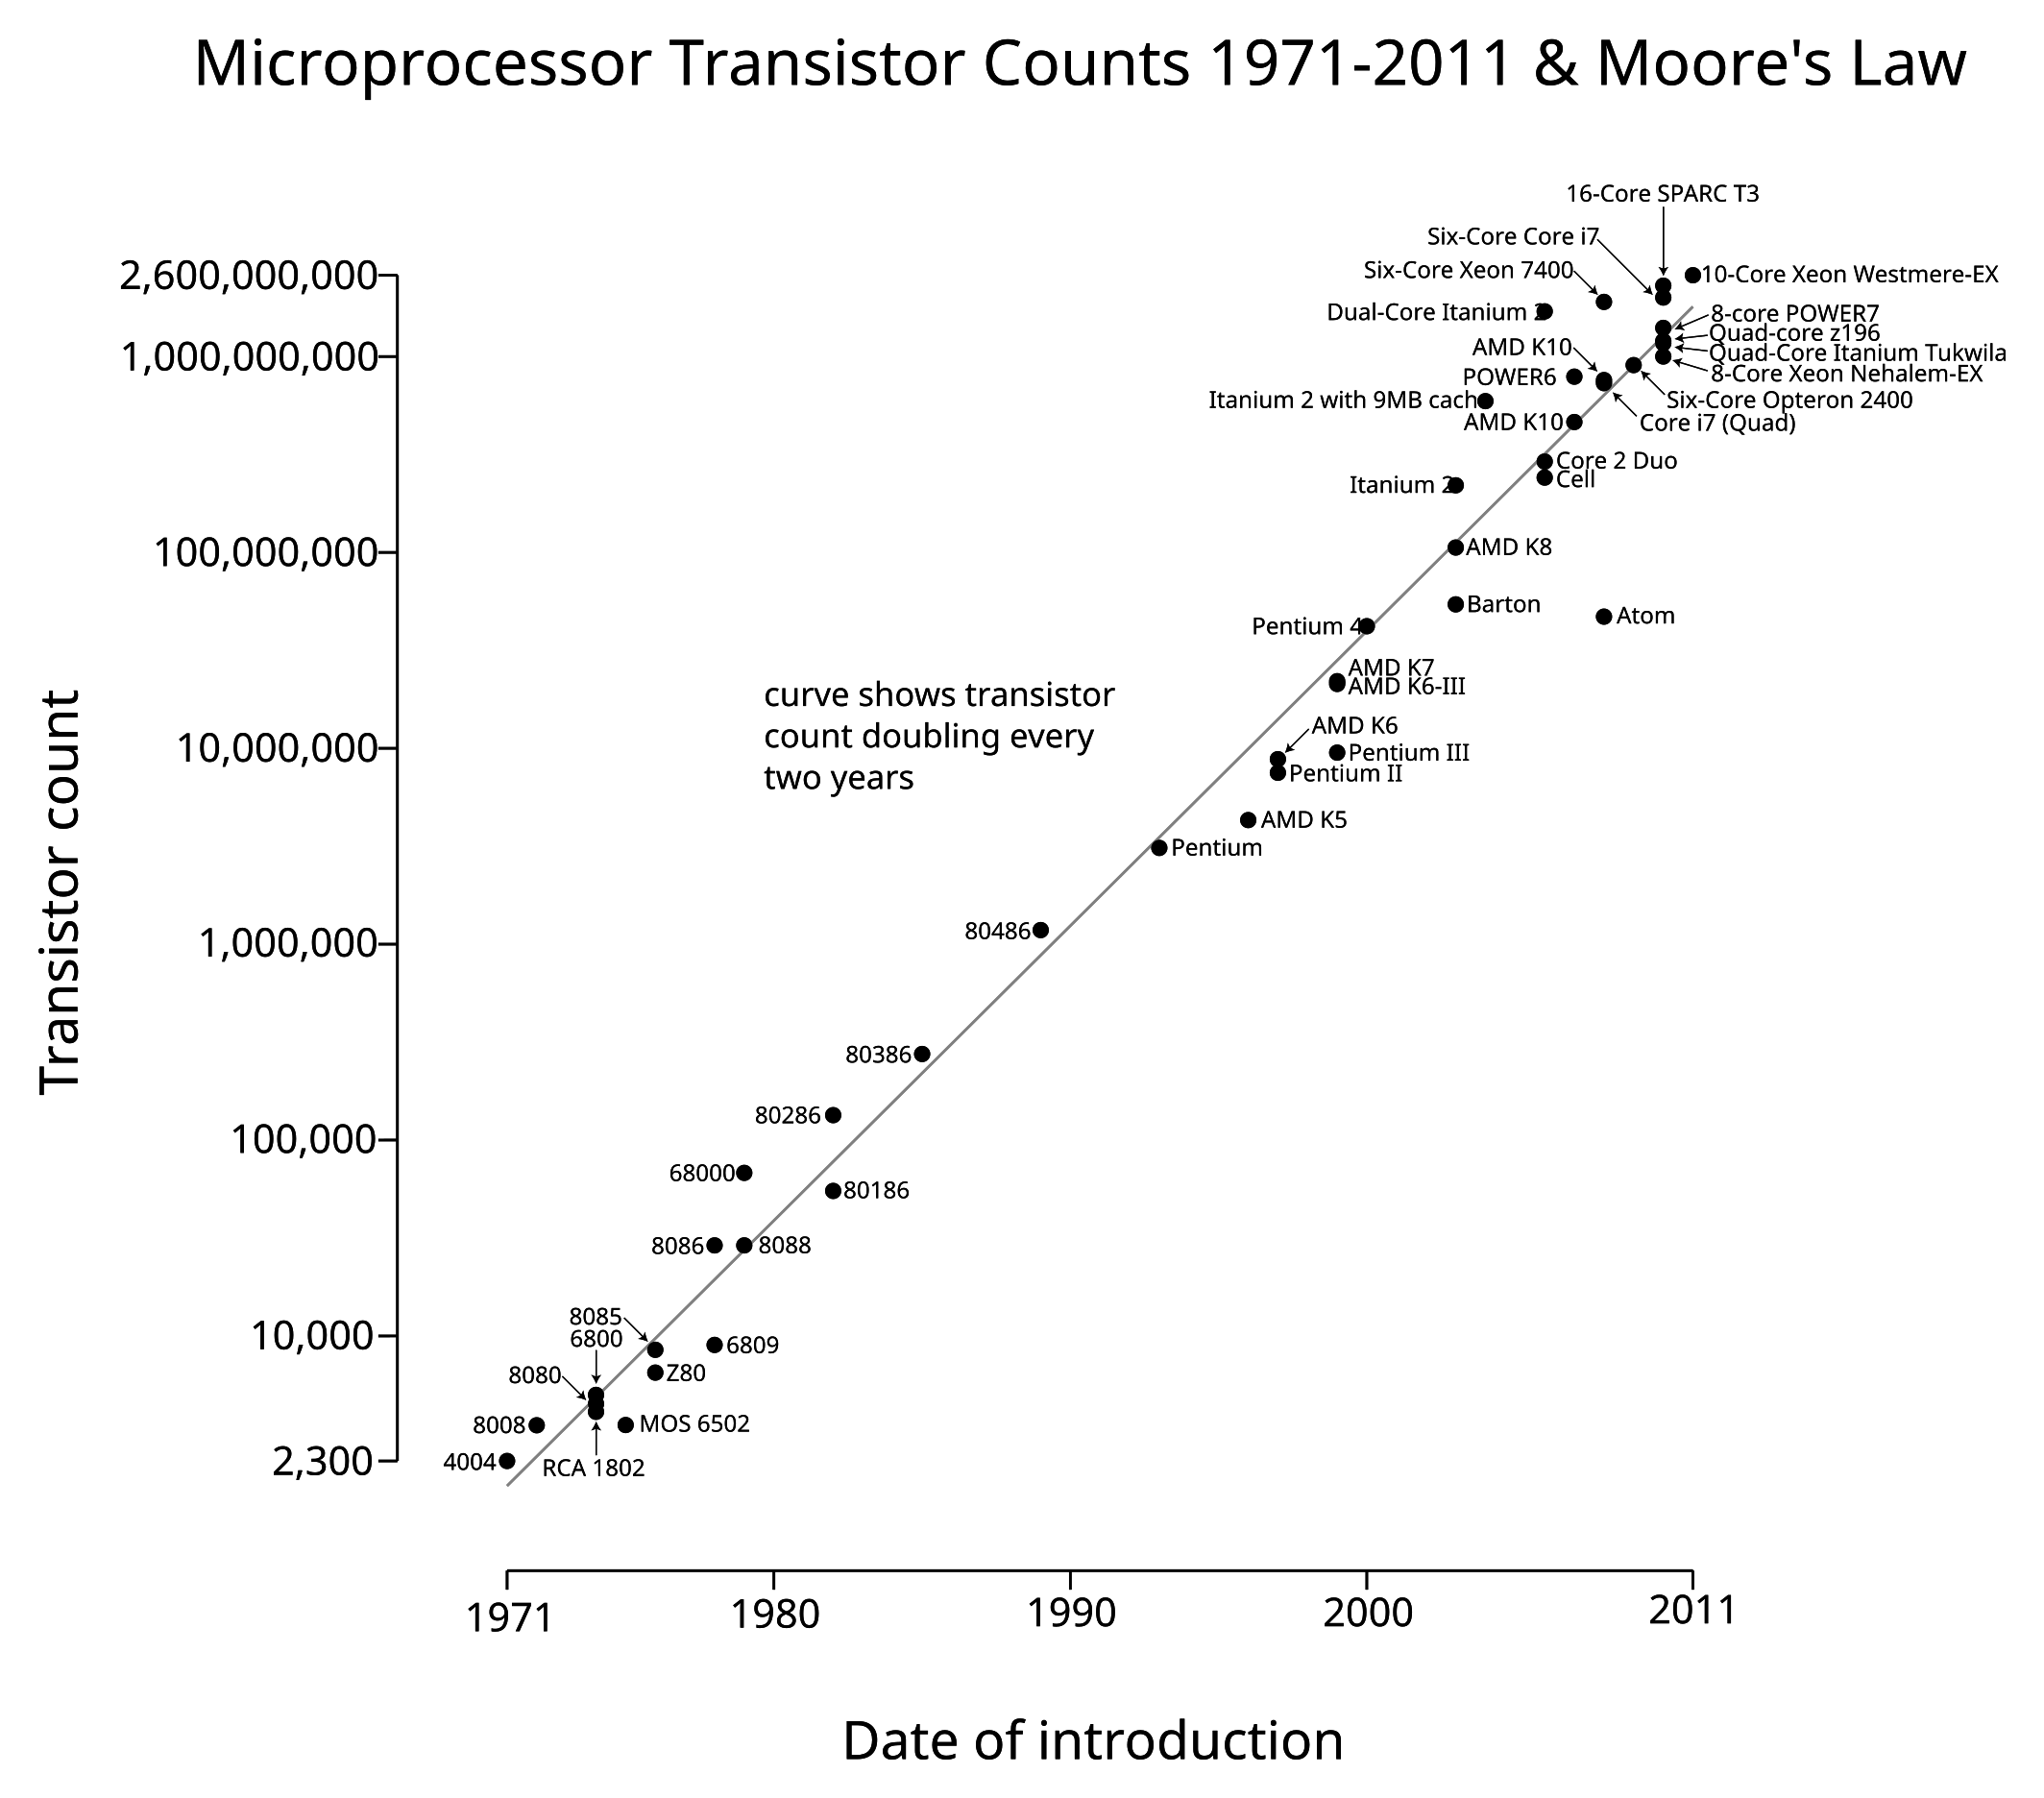
\includegraphics[width=0.48\linewidth]{moore.png}

\vspace{0.6em}
\small
一款现代手机 SoC 包含百亿级晶体管。\\[0.2em]
问题不再只是``功能能不能做出来''，而是``这个功能能否被组织成清楚、稳定、可验证、可修改的结构''。

\vspace{0.4em}
\textbf{结论}：现代芯片设计必须依赖抽象与分层。
\end{frame}

\begin{frame}{Abstraction Hierarchy}
\centering
\setlength{\tabcolsep}{10pt}
\renewcommand{\arraystretch}{0.85}
\begin{tabular}{@{}c c@{}}
\raisebox{-0.5\height}{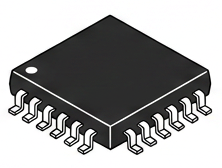
\includegraphics[width=1.1cm]{system.png}}  & \raisebox{-0.5\height}{\textbf{System / 系统层}} \\
                                                                    & {\small $\Uparrow$}                               \\
\raisebox{-0.5\height}{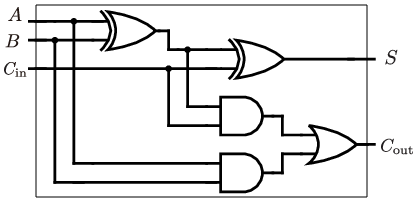
\includegraphics[width=1.1cm]{module.png}}  & \raisebox{-0.5\height}{\textbf{Module / 模块层}} \\
                                                                    & {\small $\Uparrow$}                               \\
\raisebox{-0.5\height}{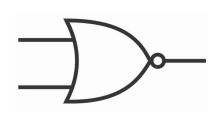
\includegraphics[width=1.1cm]{gate.png}}    & \raisebox{-0.5\height}{\textbf{Gate / 逻辑门层}} \\
                                                                    & {\small $\Uparrow$}                               \\
\raisebox{-0.5\height}{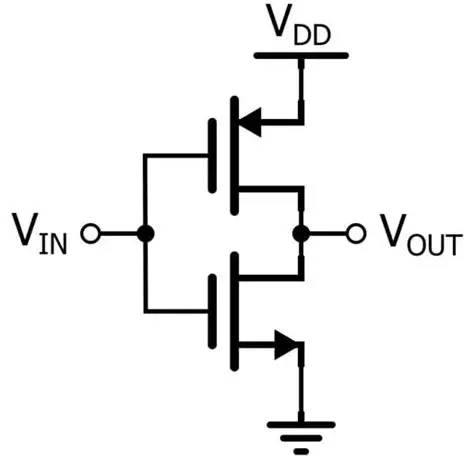
\includegraphics[width=1.1cm]{circuit.png}} & \raisebox{-0.5\height}{\textbf{Circuit / 电路层}} \\
                                                                    & {\small $\Uparrow$}                               \\
\raisebox{-0.5\height}{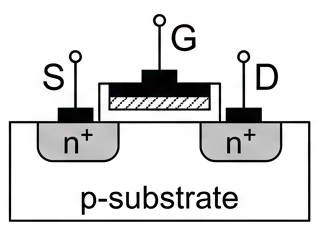
\includegraphics[width=1.1cm]{nmos.png}}    & \raisebox{-0.5\height}{\textbf{Device / 器件层}}
\end{tabular}

\vspace{0.5em}
\footnotesize
每一层只处理本层必须面对的问题，并通过接口把复杂性隔离在边界上。
\end{frame}

\begin{frame}{The Digital Abstraction}
\begin{itemize}
  \item 真实电路处理的是连续电压、电流、延迟与噪声
  \item 数字设计把它抽象成逻辑 0 / 1、时钟边沿与状态更新
  \item 这层抽象的价值：
  \begin{itemize}
    \item 让设计可组合
    \item 让验证可分层
    \item 让团队能够协作
  \end{itemize}
  \item 这层抽象的前提：
  \begin{itemize}
    \item 电平必须可靠
    \item 时序必须满足
    \item 接口边界必须清楚
  \end{itemize}
\end{itemize}
\end{frame}

\begin{frame}{From Physics to Logic}
\small
数字抽象不是天然存在的，它是一层人工构建的逻辑秩序：

\vspace{0.5em}
\begin{itemize}
  \item 把一部分电压范围定义为逻辑 0，另一部分定义为逻辑 1
  \item 禁止长期停留在模糊区间
  \item 让组合逻辑在时钟周期内收敛，再由寄存器捕获
\end{itemize}

\vspace{0.7em}
\textbf{后面会学到的 setup / hold / metastability / protocol，都是在保护这层抽象不失效。}
\end{frame}

\begin{frame}{The Integrated Circuit Era}
\centering
\begin{columns}[T]
  \column{0.48\linewidth}
  \centering
  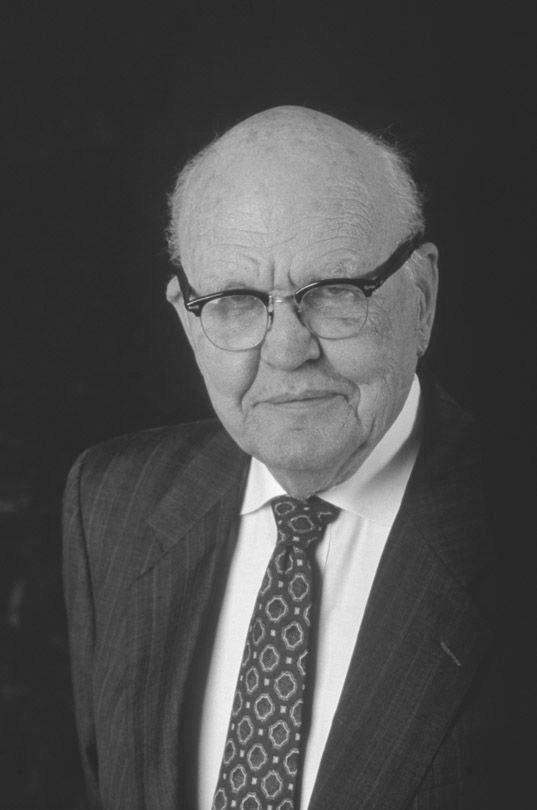
\includegraphics[width=0.65\linewidth]{kilby.jpg}

  \vspace{0.3em}
  \scriptsize Jack Kilby，1958

  \vspace{0.5em}
  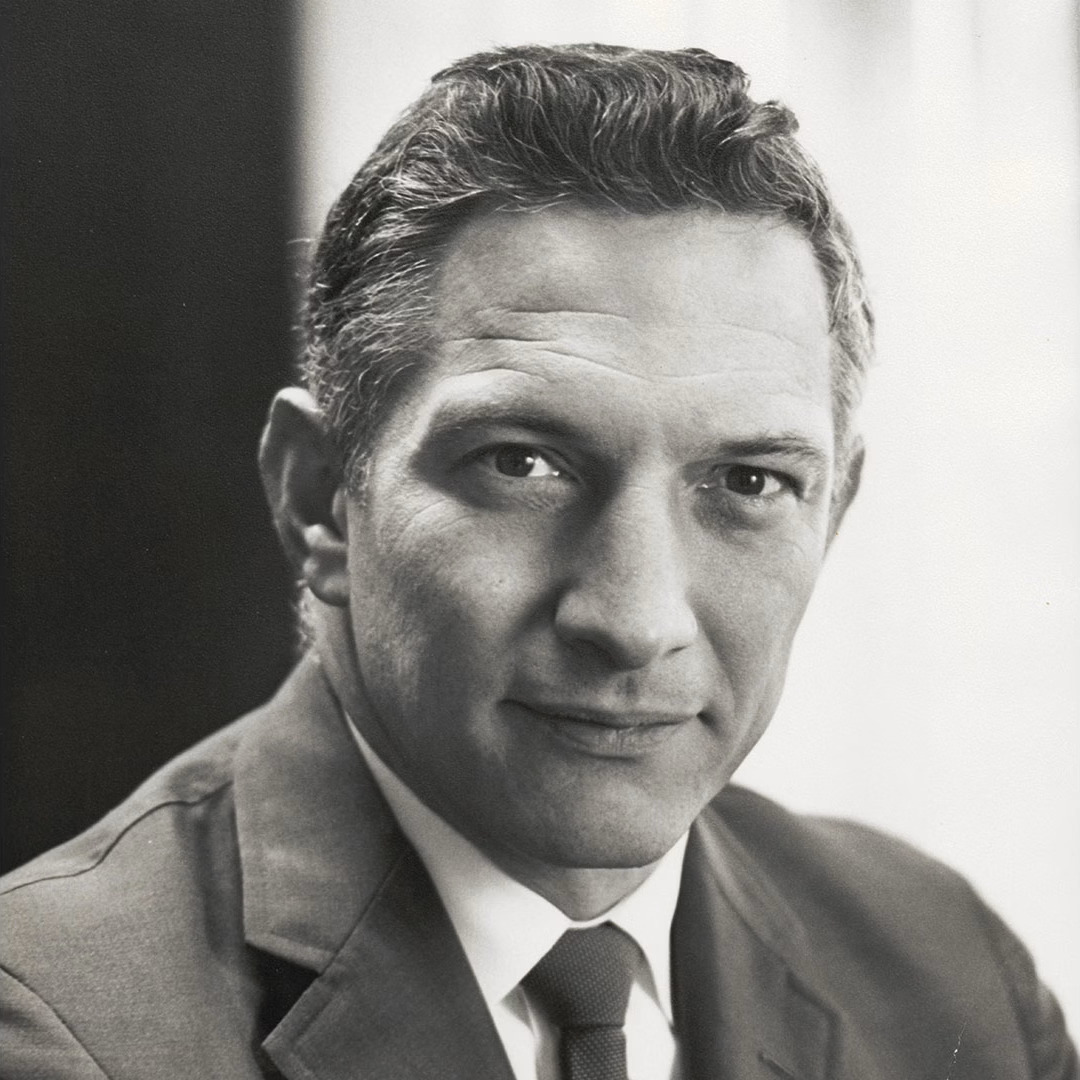
\includegraphics[width=0.65\linewidth]{noyce.jpg}

  \vspace{0.3em}
  \scriptsize Robert Noyce，1959

  \column{0.48\linewidth}
  \small
  \begin{itemize}
    \item Kilby 与 Noyce 共同开启集成电路时代
    \item Noyce 的硅平面工艺更适合大规模制造
    \item 关键变化不是``发明了一个新器件''
    \item 而是：电子工程的默认起点开始从\textbf{分立范式}转向\textbf{集成范式}
  \end{itemize}
\end{columns}
\end{frame}

\begin{frame}{Analog Is Also Integrated}
\begin{columns}[T]
  \column{0.42\linewidth}
  \centering
  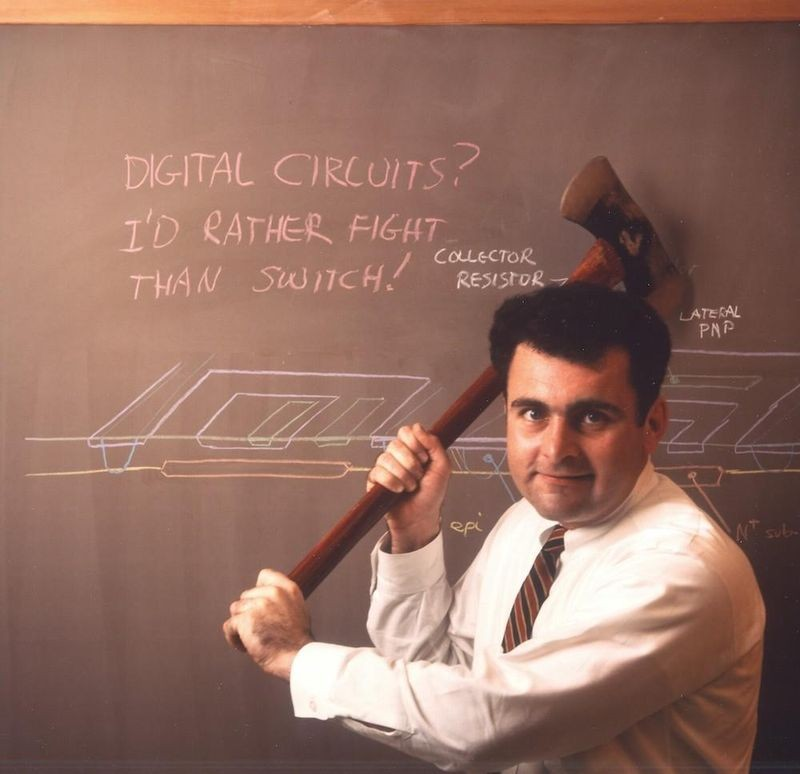
\includegraphics[width=0.72\linewidth]{widlar.jpg}

  \vspace{0.4em}
  \scriptsize Robert Widlar (1937--1991)

  \vspace{0.3em}
  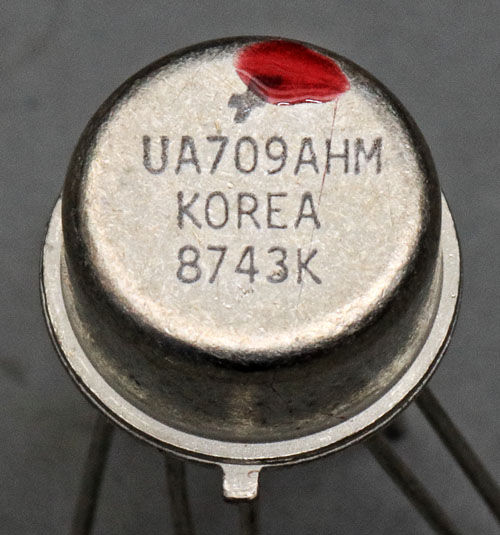
\includegraphics[width=0.24\linewidth]{ua709.jpg}

  \vspace{0.2em}
  \scriptsize \textmu A709 单片运放
  \column{0.54\linewidth}
  \small
  \begin{itemize}
    \item Widlar 的意义，不只是一个传奇人物
    \item 而是说明：\textbf{模拟电路同样被集成化重塑}
    \item 从单片运放到今天的 ADC、PMIC、driver 芯片
    \item 模拟、数字、混合信号都在走向更高集成度
  \end{itemize}

  \vspace{0.4em}
  \footnotesize
  历史在这里是证据：集成化不是数字世界的特例，而是现代电子工程的共同方向。
\end{columns}
\end{frame}

\begin{frame}{From Discrete Circuits to SoC}
\centering
\begin{columns}[T]
  \column{0.48\linewidth}
  \centering
  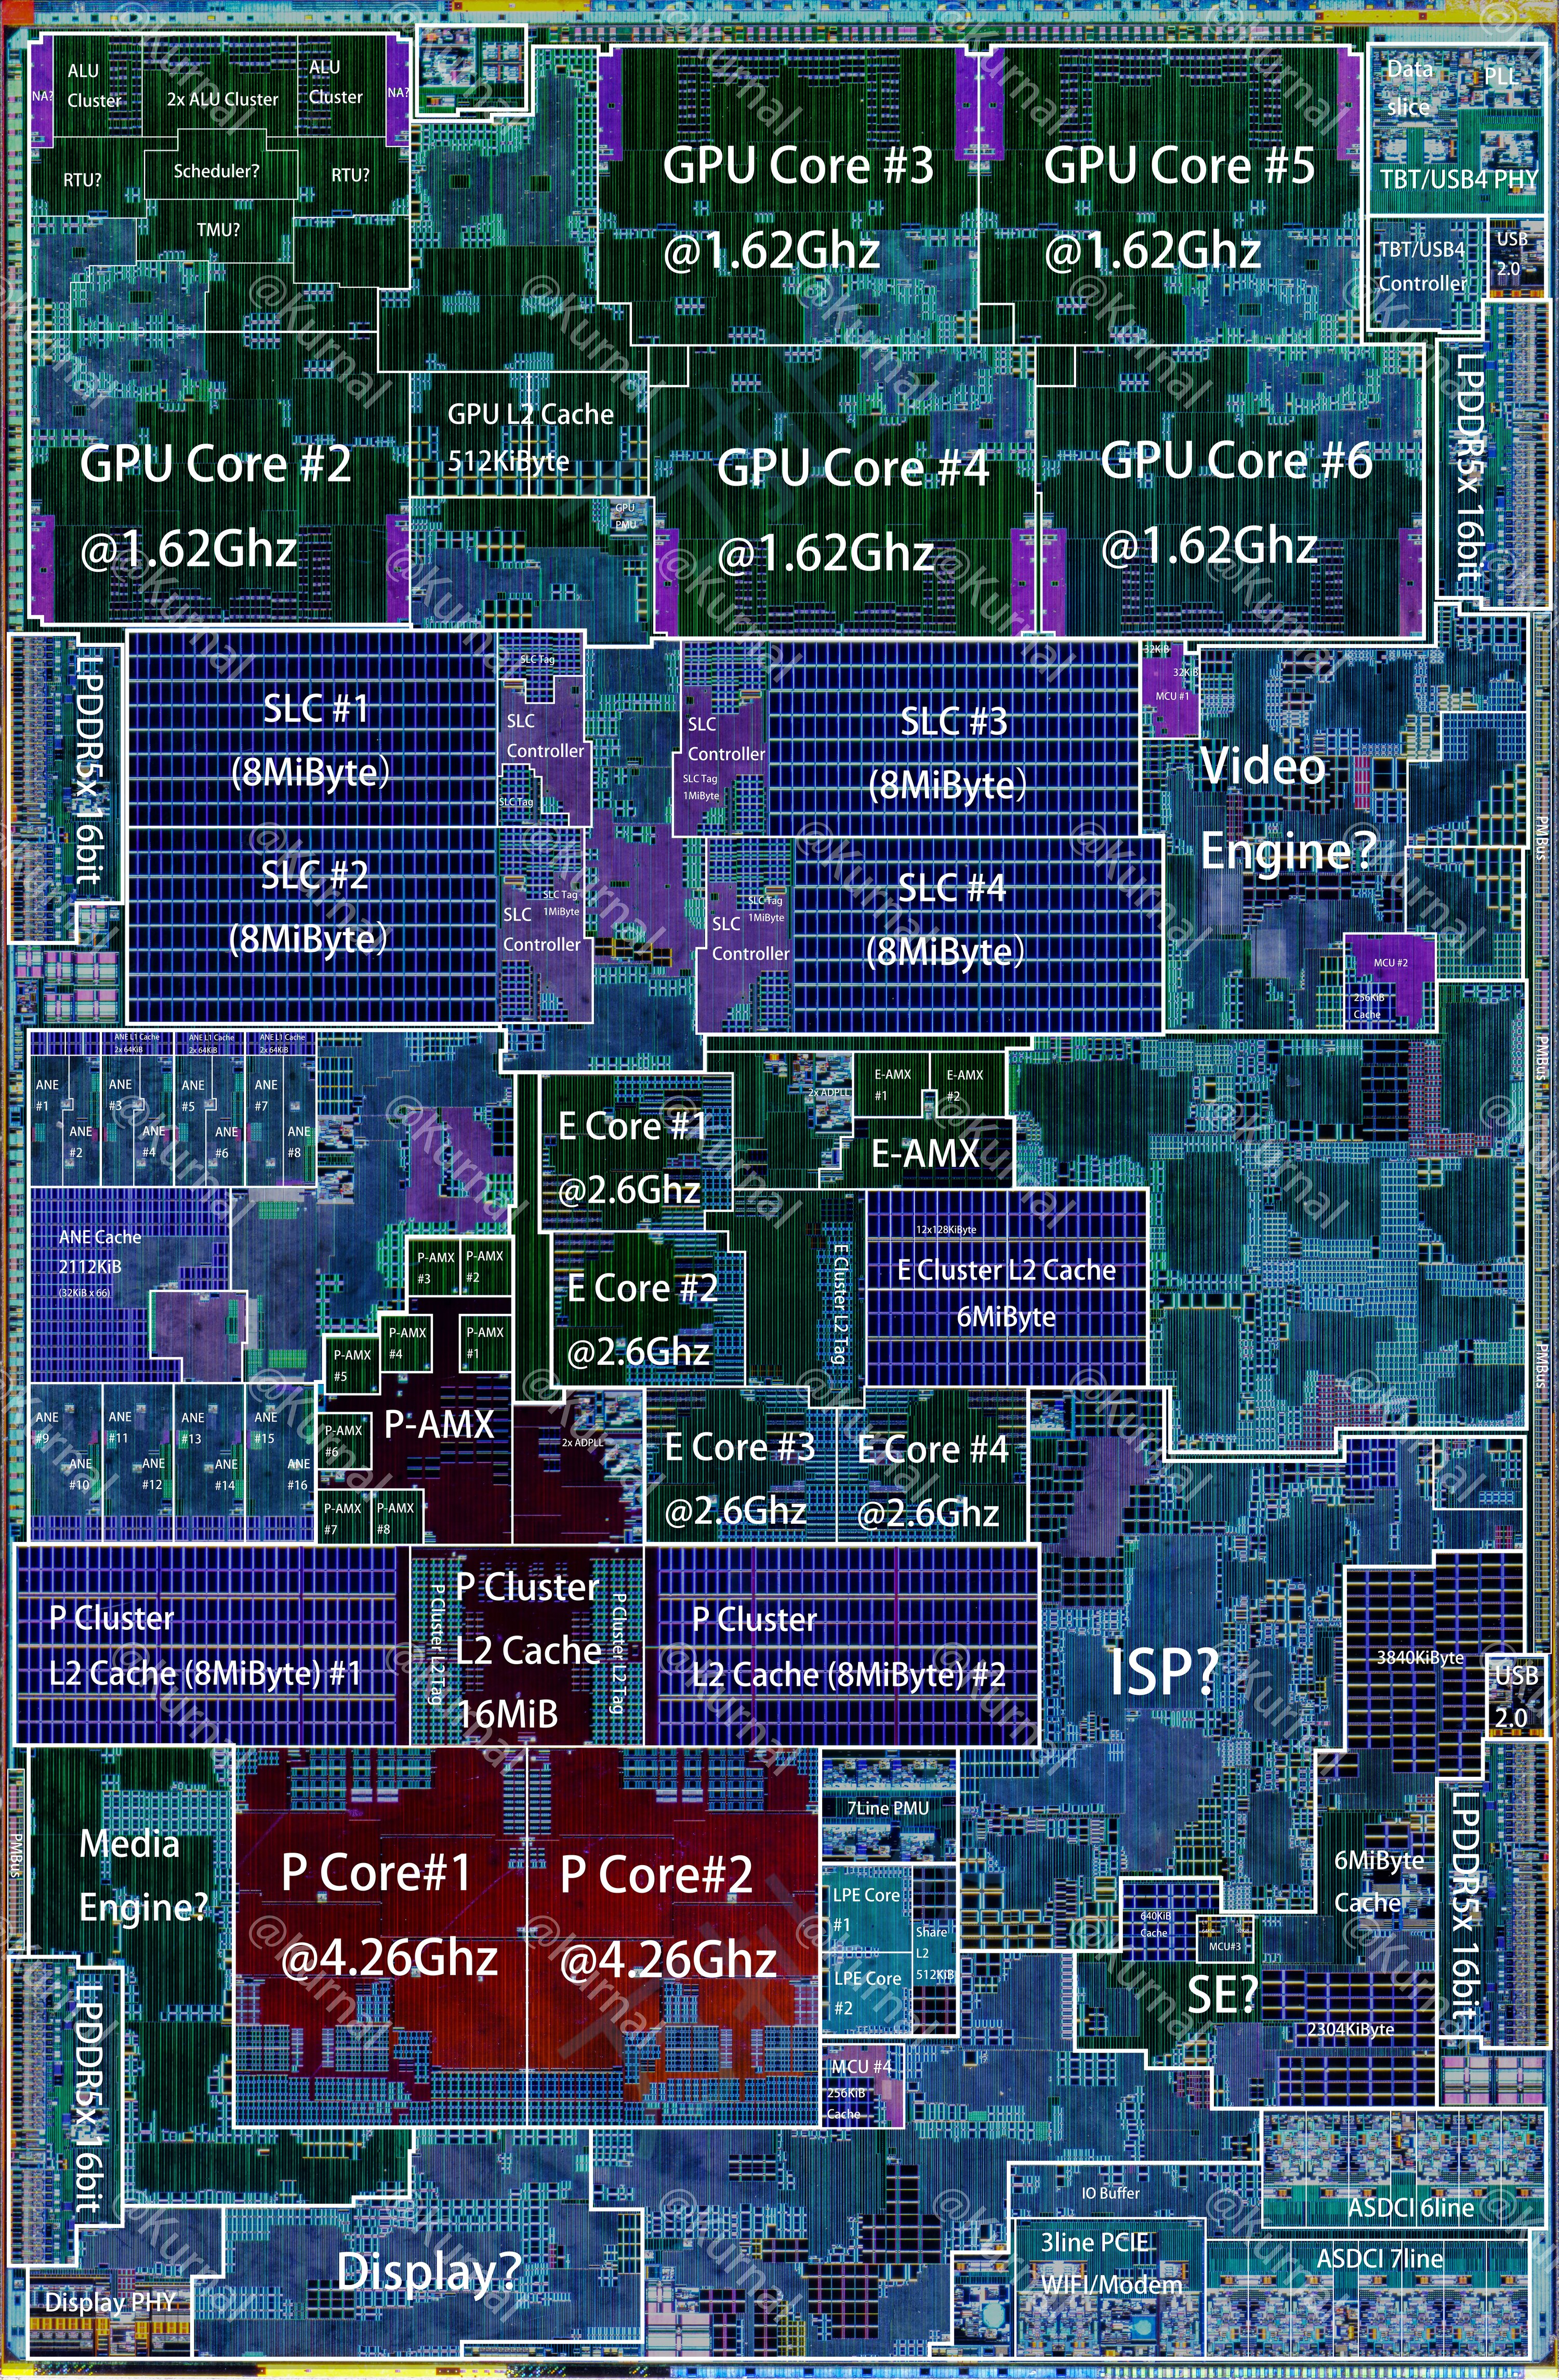
\includegraphics[width=0.7\linewidth]{a19p-layout.jpg}

  \vspace{0.3em}
  \scriptsize 现代数字 SoC：CPU + GPU + NPU + ISP + 基带...
  \column{0.48\linewidth}
  \centering
  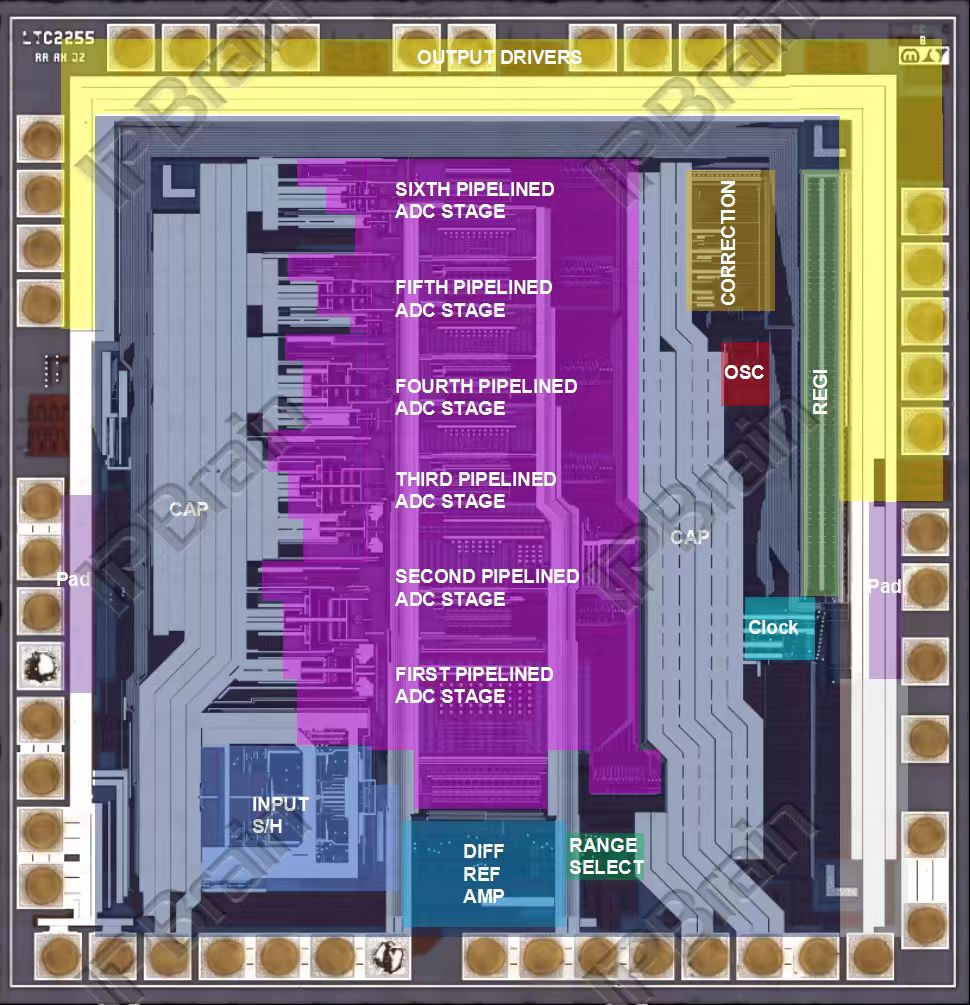
\includegraphics[width=0.88\linewidth]{adc_layout.jpg}

  \vspace{0.3em}
  \scriptsize 现代模拟 / 混合信号芯片：模拟前端 + 数字校准 + 接口...
\end{columns}

\vspace{0.6em}
\small
\textbf{结论}：今天电子工程的默认起点，是在芯片级完成高度集成，再把这些集成器件组织成系统。
\end{frame}

\begin{frame}{SoC Methodology and Complete Solutions}
\begin{itemize}
  \item SoC 不只是``一种芯片''，而是一种系统构建范式
  \item IP 复用让设计公司不必从零开发每个子系统
  \item 典型积木：CPU 核、DDR / USB / PCIe PHY、ADC、PLL、存储控制器
  \item 芯片公司还会提供完整方案：
  \begin{itemize}
    \item 参考设计、评估板、原理图
    \item 在线设计工具和参数计算工具
    \item 应用文档、软件库和支持体系
  \end{itemize}
\end{itemize}

\vspace{0.4em}
\footnotesize
现代工程师越来越少``从分立元件重新搭系统''，越来越多是在做选型、参数配置与系统整合。
\end{frame}

\begin{frame}{From Die to System}
\begin{columns}[T]
  \column{0.48\linewidth}
  \centering
  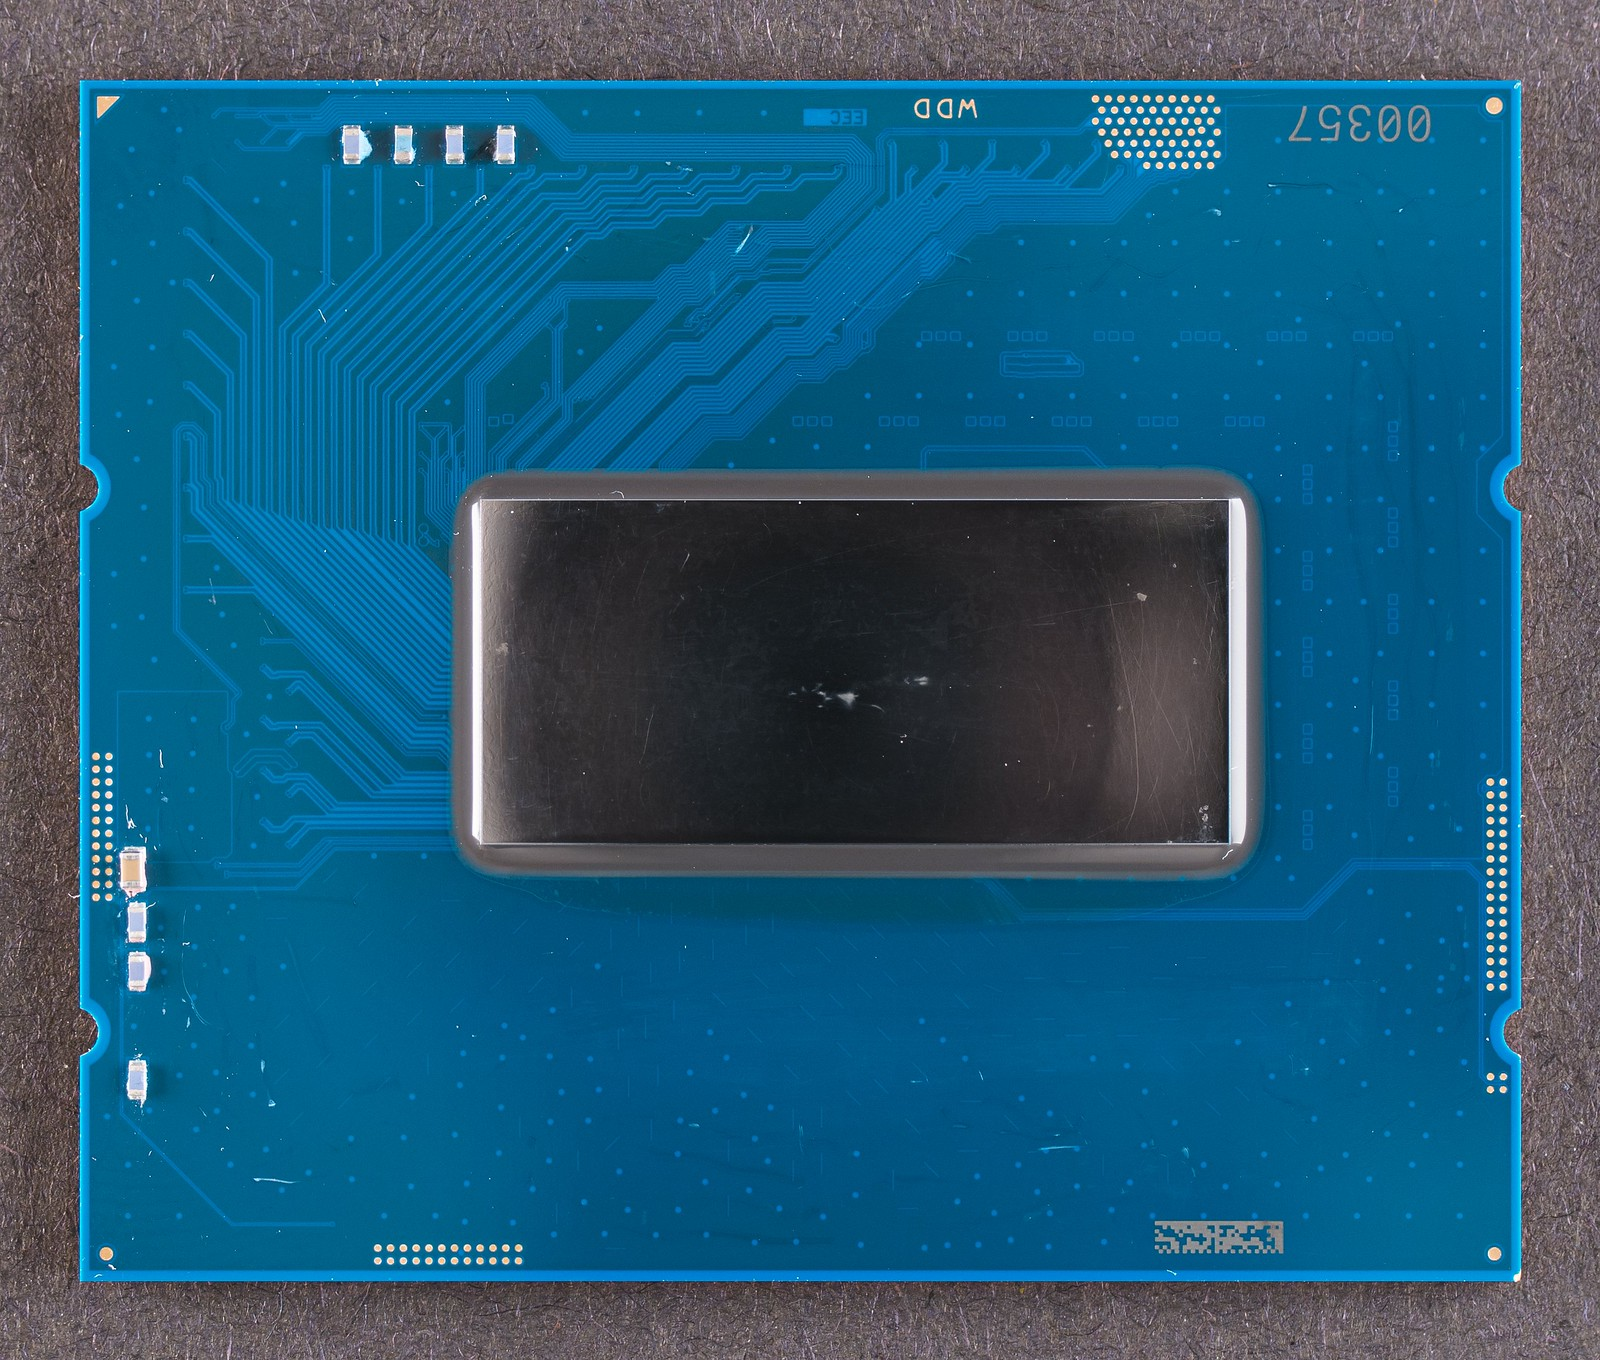
\includegraphics[width=0.55\linewidth]{silicon_chip.jpg}

  \vspace{0.4em}
  \scriptsize 封装后的芯片（chip）

  \vspace{0.6em}
  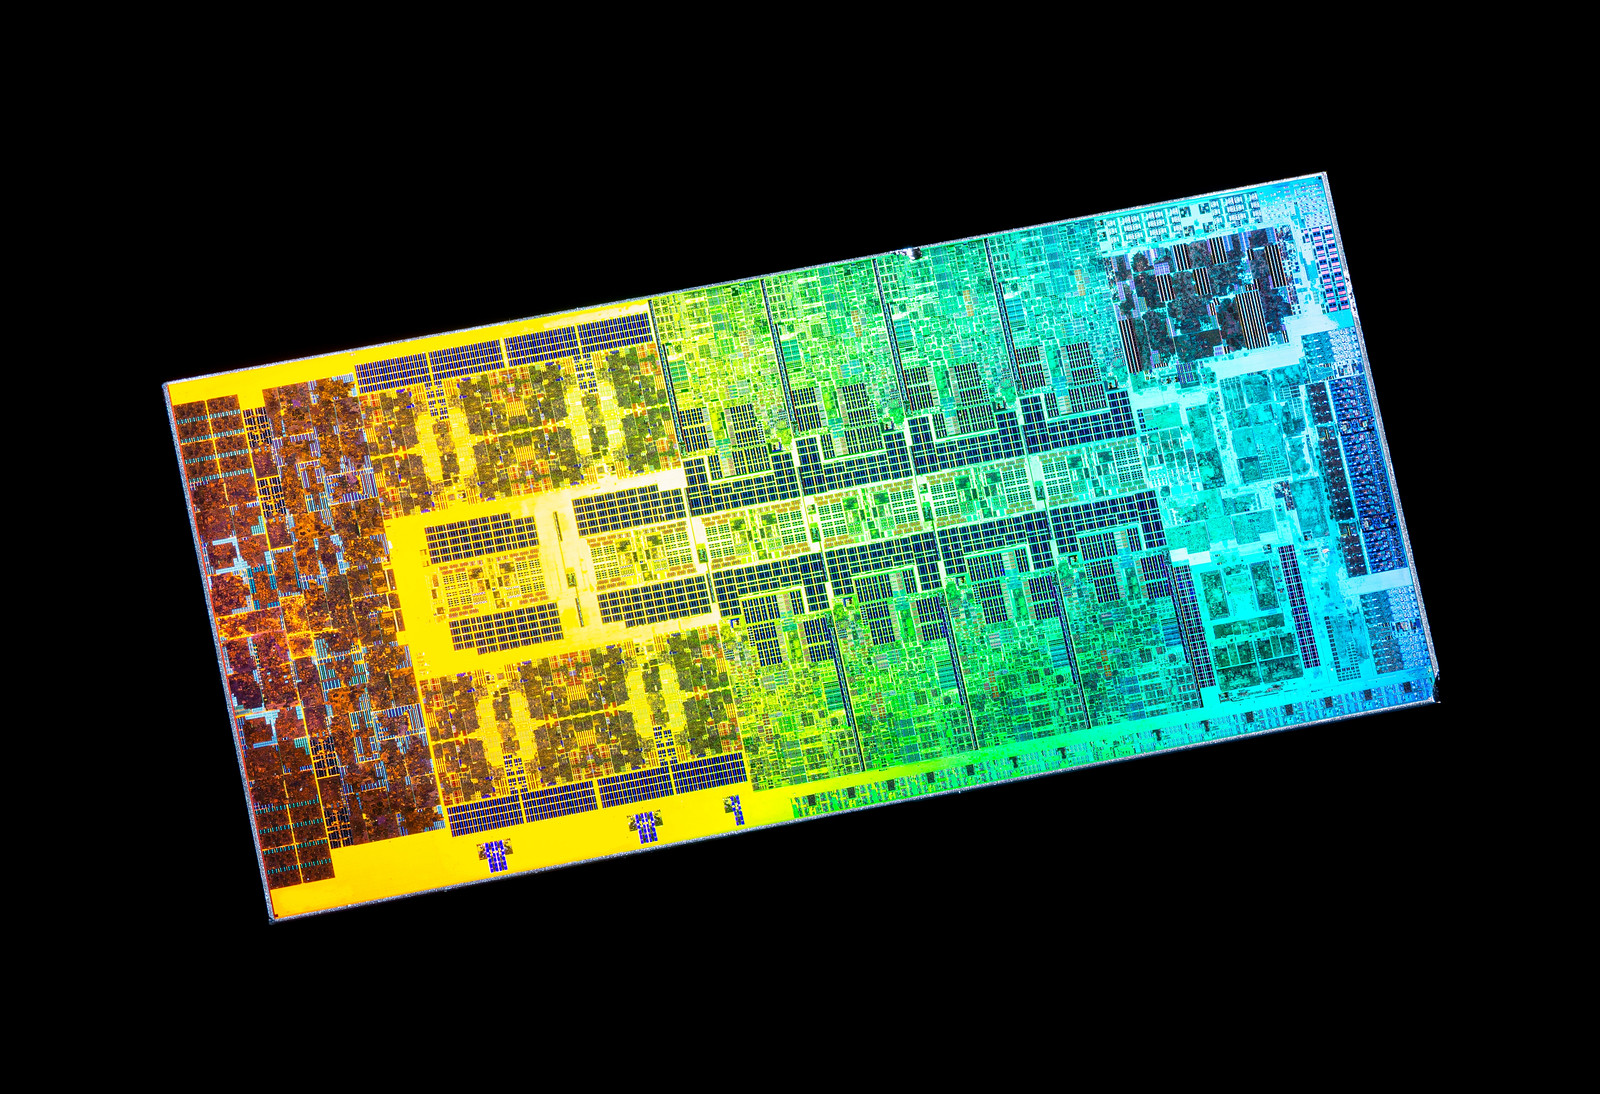
\includegraphics[width=0.50\linewidth]{silicon_die.jpg}

  \vspace{0.4em}
  \scriptsize 尚未封装的裸片（die）
  \column{0.48\linewidth}
  \begin{itemize}
    \item \texttt{die}：制造完成但尚未封装的裸片
    \item \texttt{package}：提供保护、电连接与散热路径
    \item \texttt{chip}：工程语境中常指可上板使用的封装器件
    \item \texttt{board}：多个器件焊接在 PCB 上形成板级系统
    \item \texttt{system}：板卡、软件、接口与外设共同工作的整体
  \end{itemize}
\end{columns}
\end{frame}

\begin{frame}{Why Packaging Exists}
\begin{columns}[T]
  \column{0.55\linewidth}
  \centering
  \begin{tabular}{ccc}
  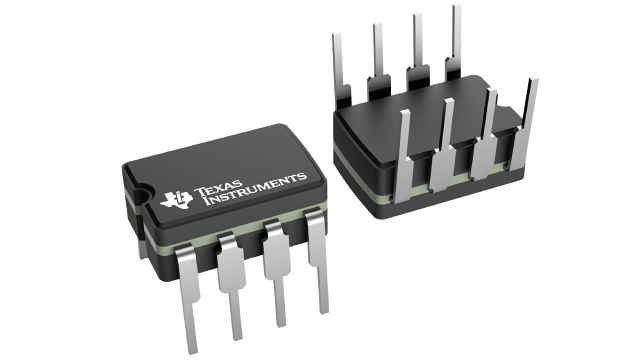
\includegraphics[width=0.22\linewidth]{DIP.png} &
  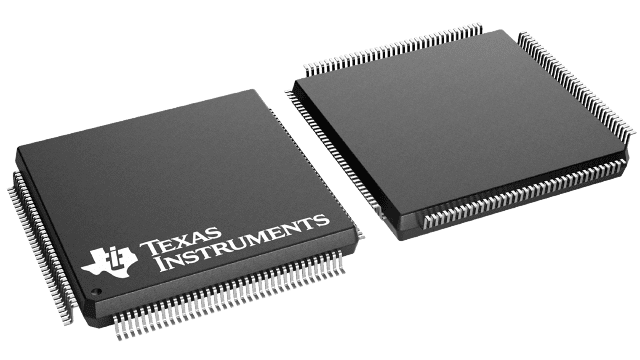
\includegraphics[width=0.22\linewidth]{QFP.png} &
  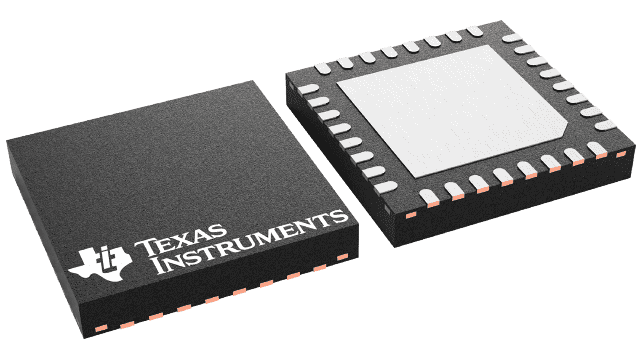
\includegraphics[width=0.22\linewidth]{QFN.png} \\
  \scriptsize DIP & \scriptsize QFP & \scriptsize QFN \\
  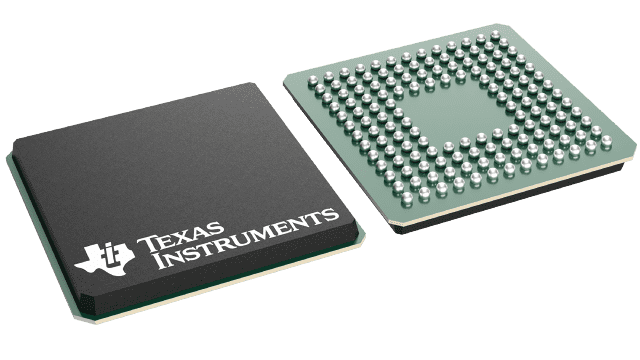
\includegraphics[width=0.22\linewidth]{BGA.png} &
  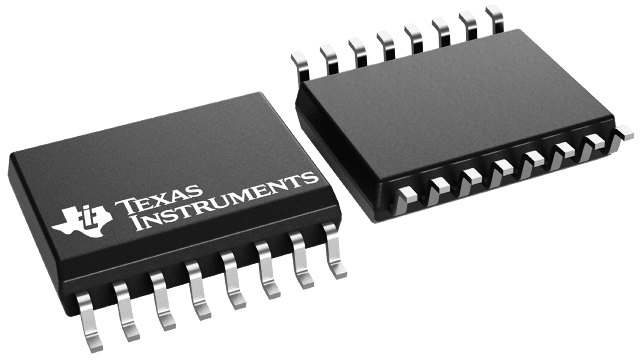
\includegraphics[width=0.22\linewidth]{SO.png} &
  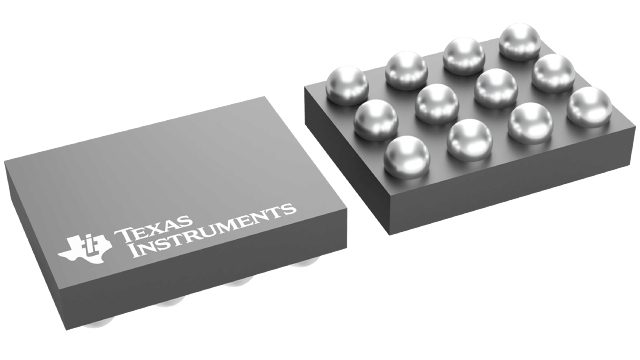
\includegraphics[width=0.22\linewidth]{DSBGA.png} \\
  \scriptsize BGA & \scriptsize SO & \scriptsize DSBGA \\
  \end{tabular}
  \column{0.40\linewidth}
  \small
  \begin{itemize}
    \item 保护脆弱的裸片
    \item 把片上焊盘转换成板级可装配引脚或焊球
    \item 提供散热路径
    \item 提供测试与装配的机械形态
    \item 不同封装是在面积、成本、引脚数、散热和组装之间做权衡
  \end{itemize}
\end{columns}
\end{frame}

\begin{frame}{A Chip Never Works Alone}
\begin{columns}[T]
  \column{0.58\linewidth}
  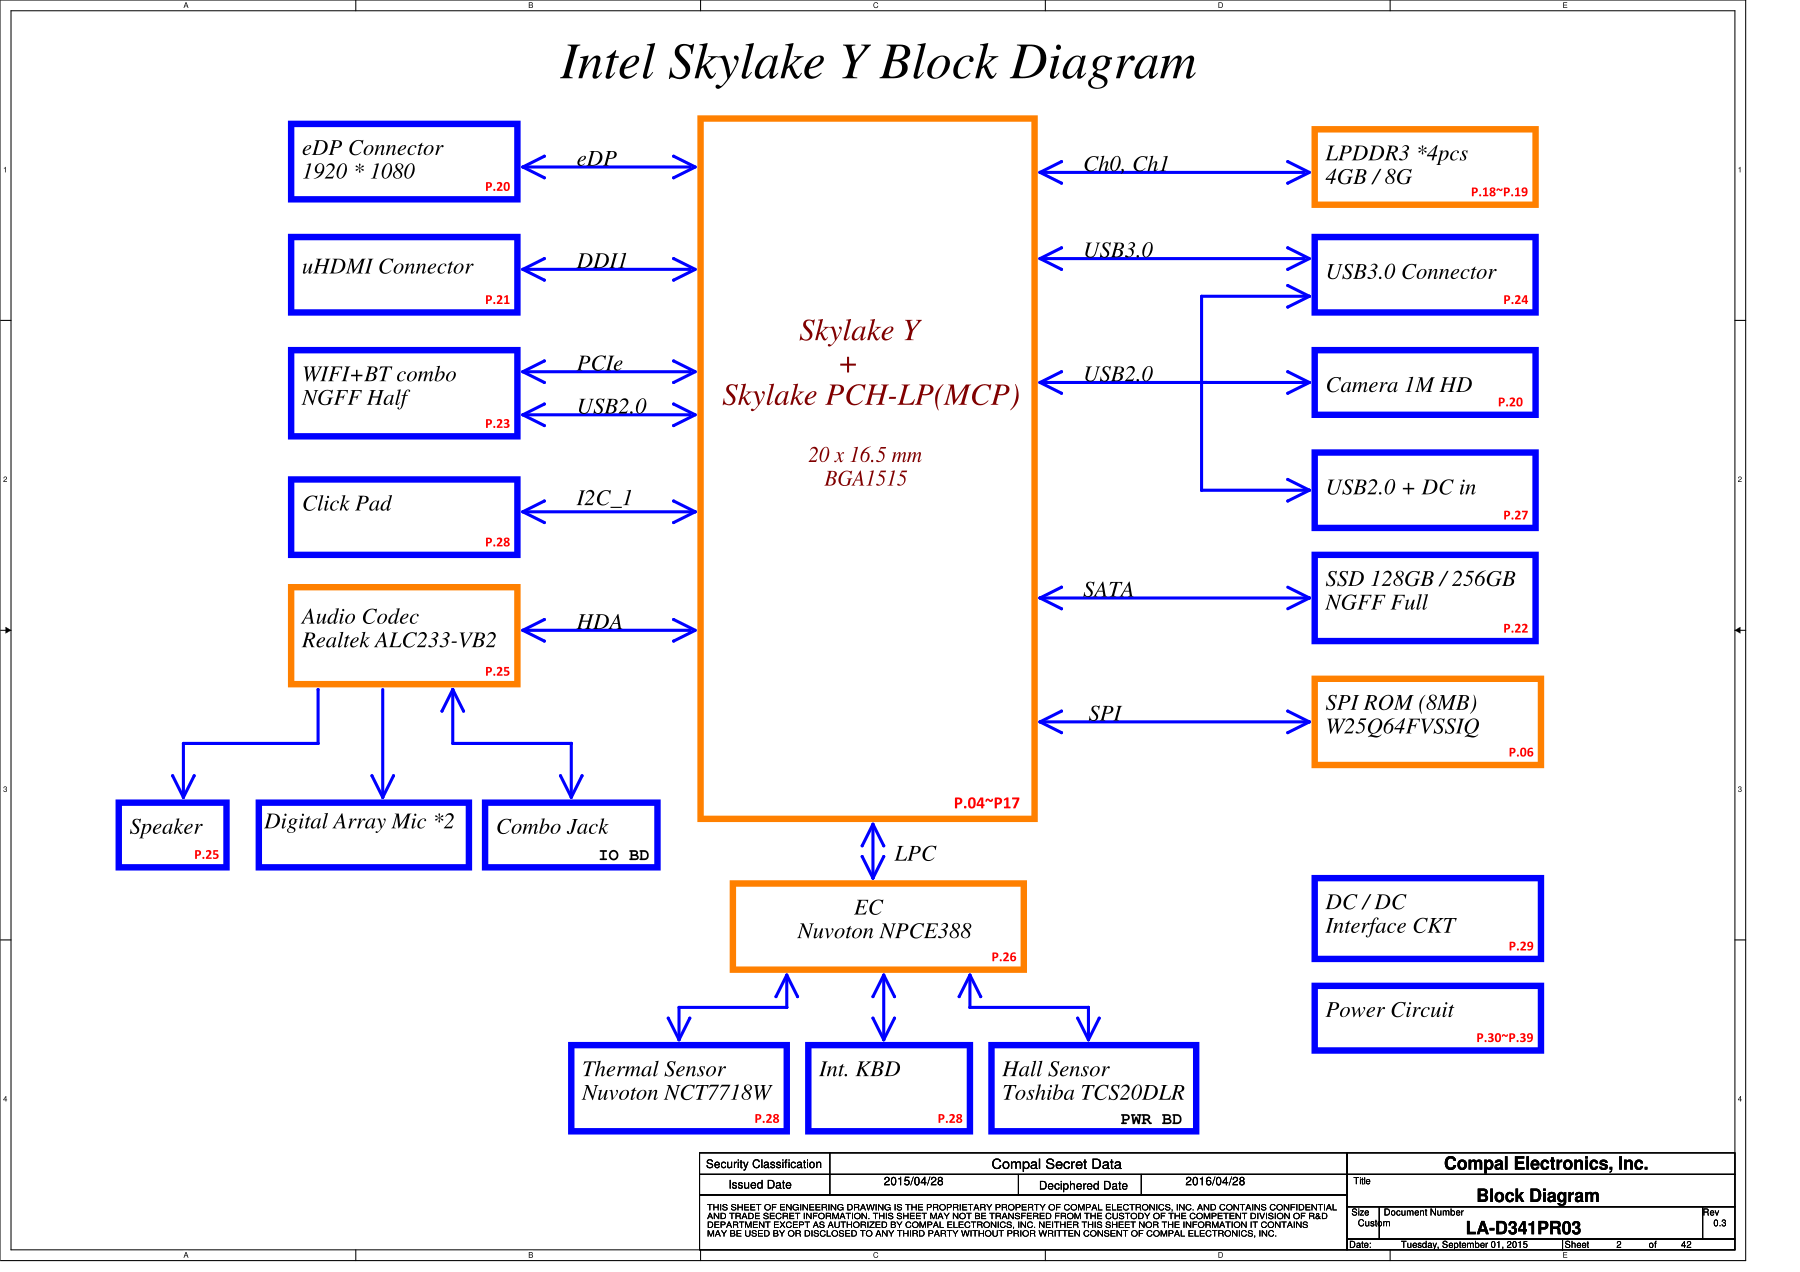
\includegraphics[width=\linewidth]{system-block-diagram.png}
  \column{0.38\linewidth}
  \small
  \begin{itemize}
    \item 主芯片需要供电网络
    \item 需要时钟和复位
    \item 需要 DRAM、Flash 等存储器配合
    \item 还要与 PMIC、接口芯片、传感器等外设协同
  \end{itemize}

  \vspace{0.5em}
  \textbf{芯片设计从来不是孤立看一颗芯片。}
\end{columns}
\end{frame}

\begin{frame}{From Block Diagram to Real Board}
\centering
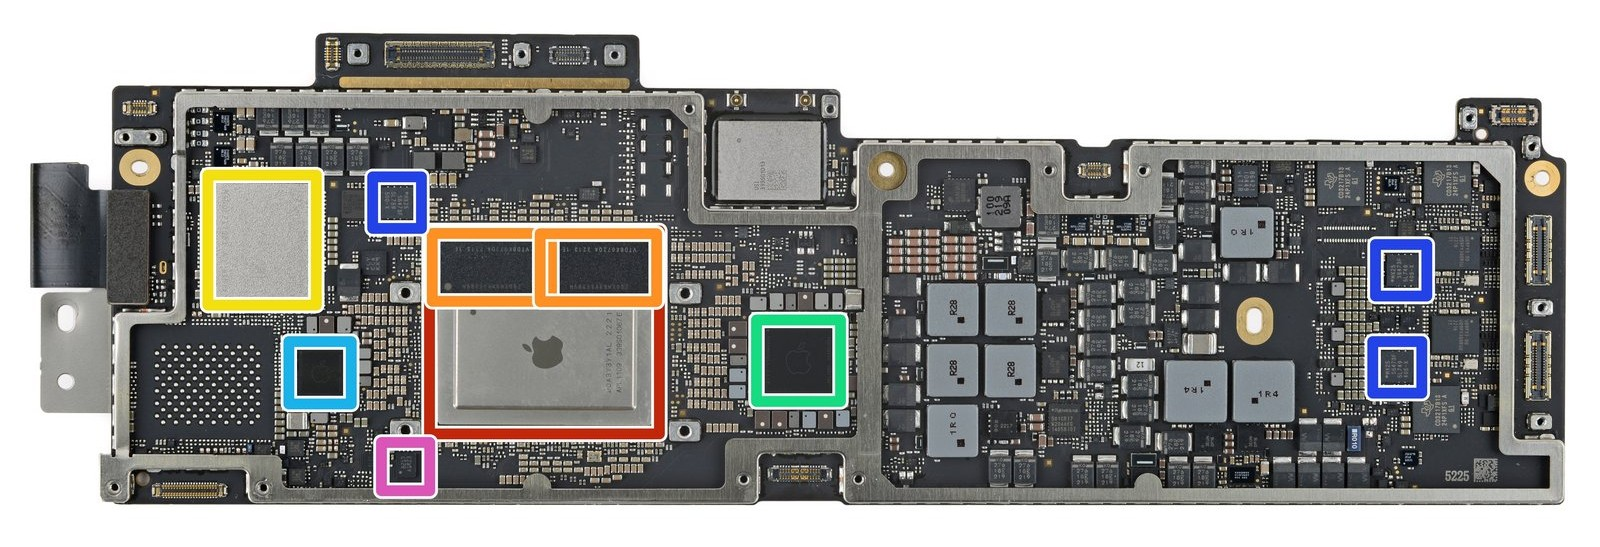
\includegraphics[width=0.92\linewidth]{mba_m2_motherboard.jpg}

\vspace{0.3em}
\small
框图是抽象的，真实主板长这样。\newline
主控、存储、电源管理与接口器件在物理上分布在不同区域，但它们共同构成一个系统。
\end{frame}

\begin{frame}{Minimal Board-Level Checklist}
\begin{itemize}
  \item 主控芯片是什么，它负责计算、控制还是接口聚合？
  \item 电源从哪里来，是否存在多个电压域？
  \item 时钟由谁提供，复位如何建立初始状态？
  \item 片外存储有哪些：DRAM、Flash、EEPROM 还是都没有？
  \item 它要和哪些外设通信：USB、PCIe、显示、传感器、网络？
\end{itemize}

\vspace{0.6em}
这 5 个问题，是你观察任何板级系统时最先应该建立的分析框架。
\end{frame}

\begin{frame}{Common Chip Types}
\centering
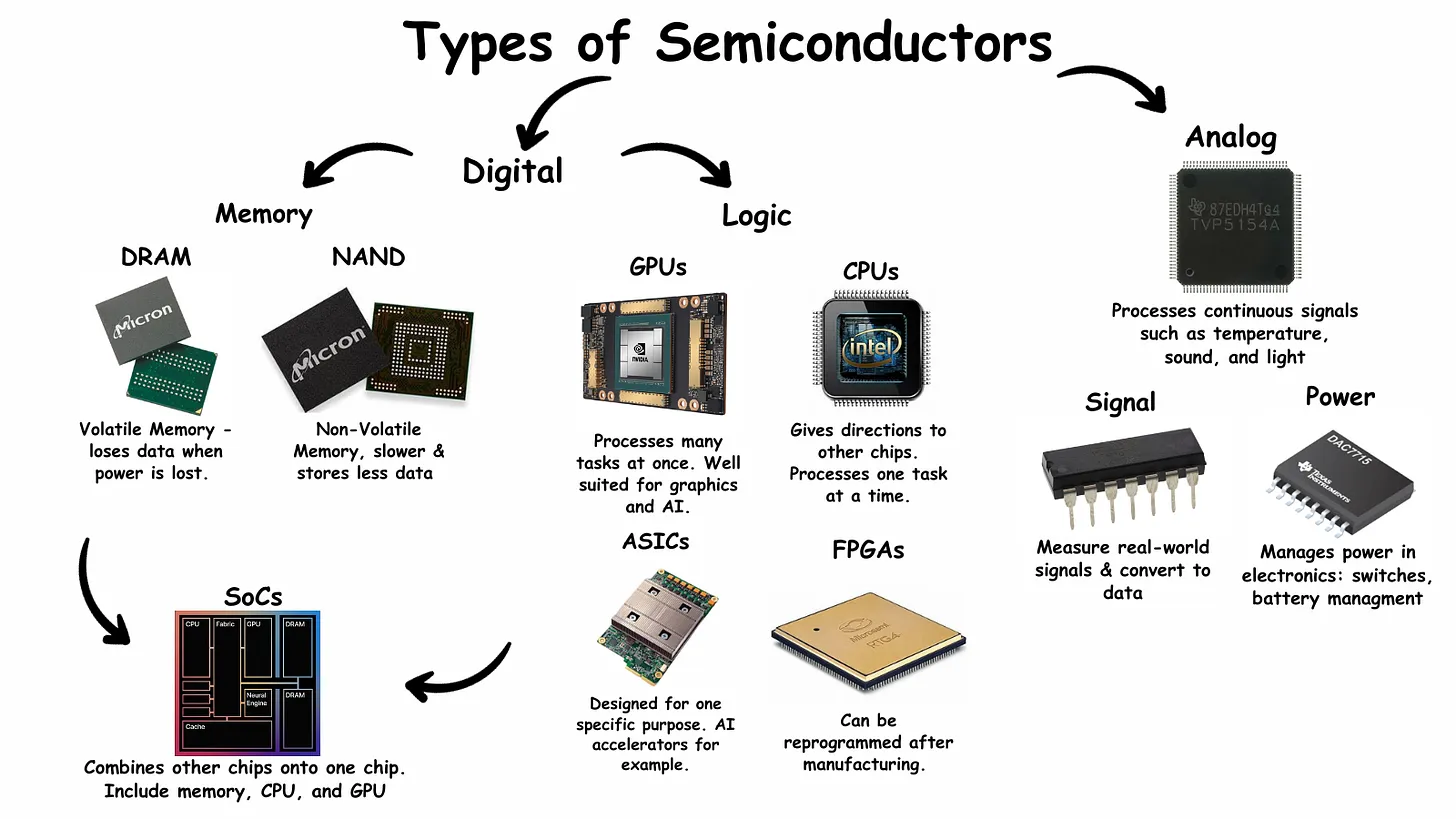
\includegraphics[width=0.74\linewidth]{type_of_chip.png}

\vspace{0.5em}
\small
分类本身不是目的，关键是理解每类芯片在系统中承担的角色：计算、控制、存储、连接、模拟与电源管理。
\end{frame}

\begin{frame}{A Simplified Digital Chip Flow}
\begin{columns}[T]
  \column{0.56\linewidth}
  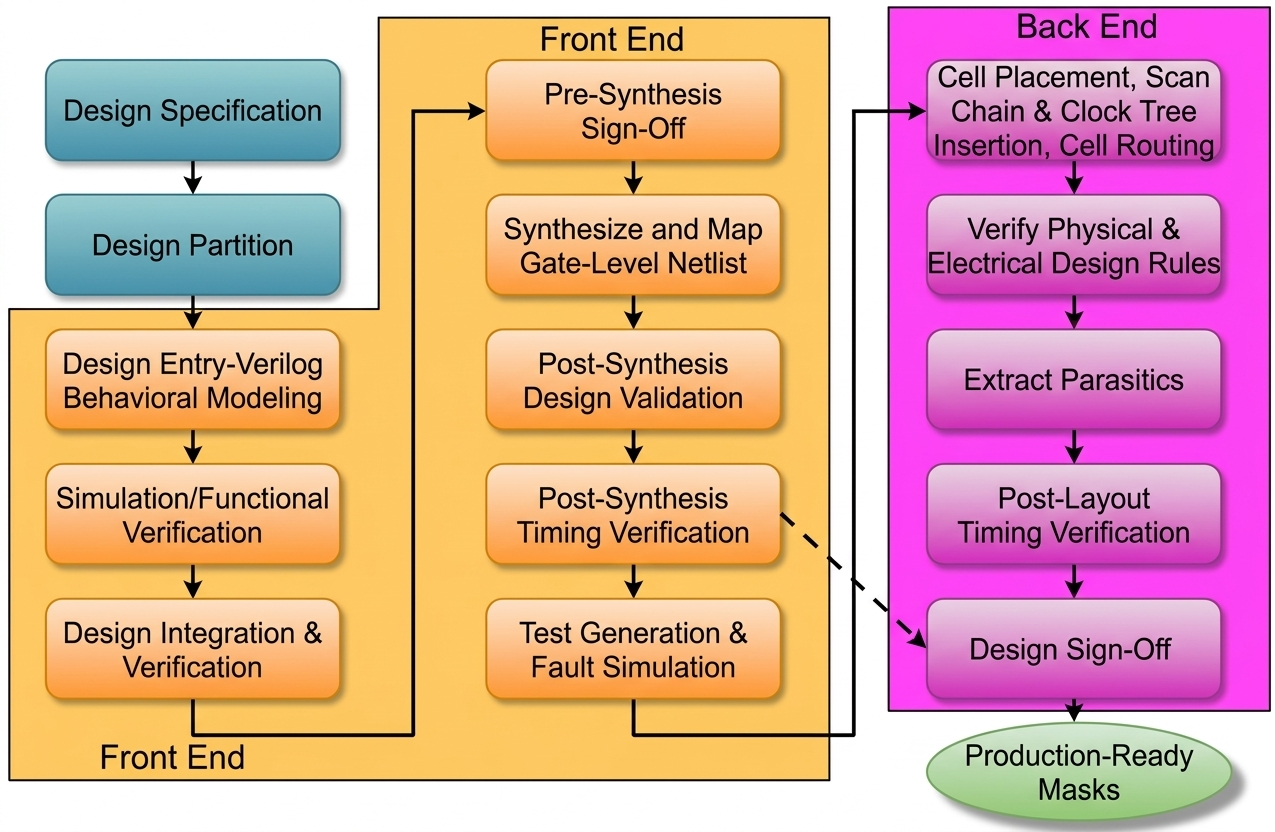
\includegraphics[width=\linewidth]{digital_flow.jpeg}
  \column{0.40\linewidth}
  \small
  \begin{itemize}
    \item Spec / Architecture
    \item RTL Design
    \item Functional Verification
    \item Synthesis
    \item Physical Design
    \item Signoff / Tapeout
  \end{itemize}

  \vspace{0.4em}
  每一步都在消费上一层抽象的结果，并生成下一层可交付物。
\end{columns}
\end{frame}

\begin{frame}{Semiconductor Ecosystem}
\centering
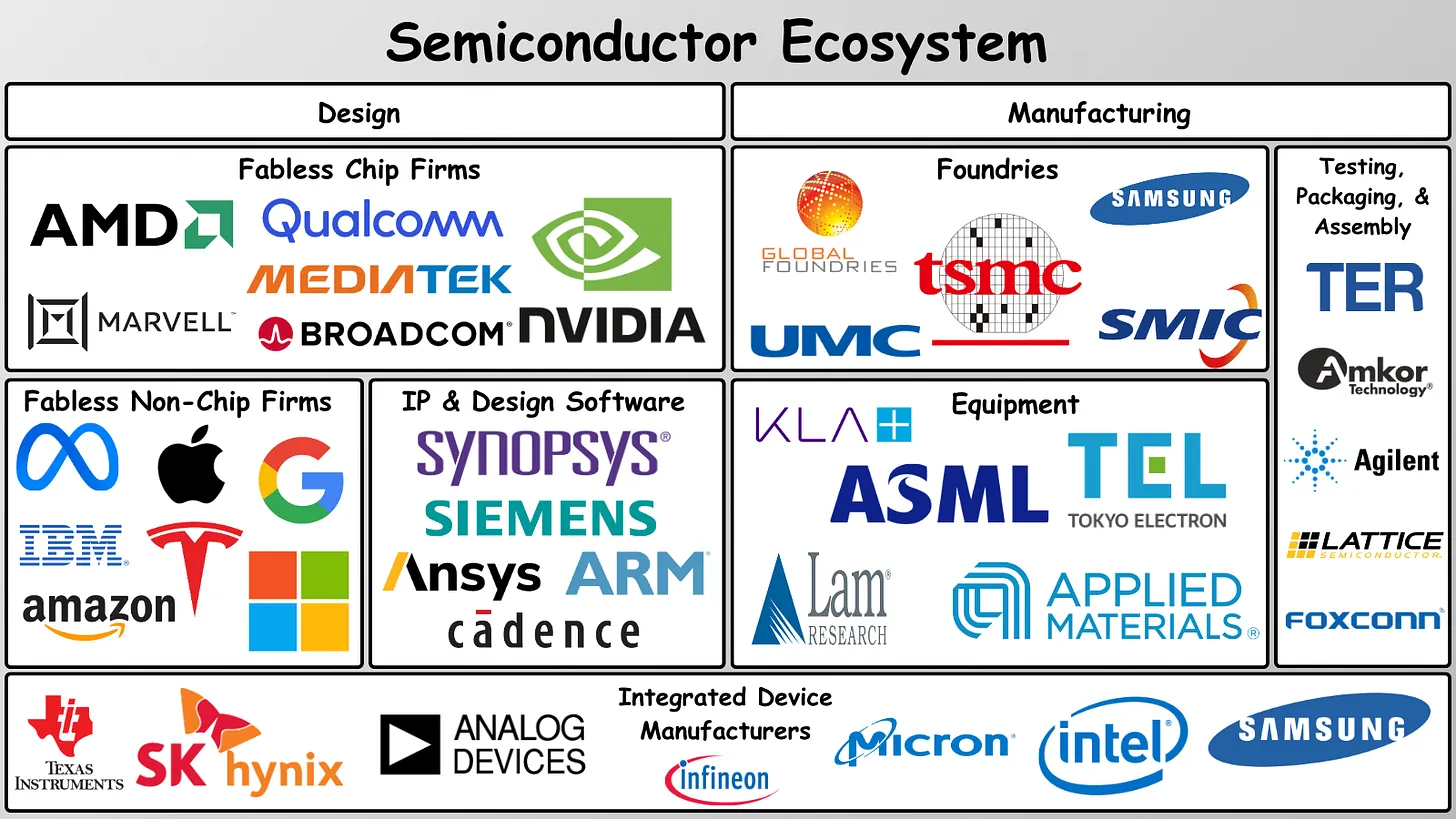
\includegraphics[width=0.76\linewidth]{semi_ecosys.png}

\vspace{0.4em}
\small
不要把所有公司都称为``芯片公司''。\newline
IP、EDA、Fabless、Foundry、OSAT、设备与材料公司解决的是不同问题。
\end{frame}

\begin{frame}{Roles and Representative Companies}
\small
读完这一章后，至少要有最基本的行业常识：

\vspace{0.4em}
\begin{itemize}
  \item \textbf{IP}：ARM、Imagination
  \item \textbf{EDA}：Synopsys、Cadence、Siemens EDA
  \item \textbf{Fabless}：NVIDIA、AMD、Qualcomm、MediaTek
  \item \textbf{Foundry}：TSMC、Samsung Foundry、SMIC
  \item \textbf{OSAT}：ASE、Amkor、长电科技
  \item \textbf{设备与材料}：ASML、Applied Materials、Lam Research
\end{itemize}

\vspace{0.4em}
\footnotesize
要求不是背大名单，而是能大致说出一家公司更像在卖 IP、卖工具、做设计、做制造，还是做封测与设备。
\end{frame}

\begin{frame}{Beyond Manufacturing}
\small
产业链主线首先是\textbf{角色分工}，但竞争不只发生在硅片制造这一层：
\begin{itemize}
  \item \textbf{TSMC}：不只做代工，也提供 PDK、设计规则和技术支持
  \item \textbf{ARM}：不只卖 IP，也提供工具、参考设计和培训生态
  \item \textbf{设计公司}：往往还提供文档、软件库、参考设计和 FAE 支持
  \item \textbf{STM32 / CUDA 这类案例}说明：很多壁垒发生在芯片之外
\end{itemize}

\vspace{0.5em}
\footnotesize
这不是说``产业链的本质只有服务竞争''，而是说：在分工结构已经成立的前提下，工具、文档、支持和生态也会显著影响竞争力。
\end{frame}

\begin{frame}{Design Rules}
\begin{itemize}
  \item \textbf{抽象优先}：先确定讨论在哪个抽象层，再谈具体方案
  \item \textbf{模块化}：把系统切成可验证、可替换、可复用的模块
  \item \textbf{接口清晰}：输入输出、时序和约束必须明确
  \item \textbf{尽早验证}：问题越晚暴露，修复代价越高
  \item \textbf{用约束管理复杂度}：面积、性能、功耗、时序是设计的一部分
\end{itemize}
\end{frame}

\begin{frame}{The 3Y Principle}
\small
面对任何模块、芯片或系统，先回答三个问题：

\vspace{0.6em}
\begin{columns}[T]
  \column{0.30\linewidth}
  \centering
  \textbf{\large Why}

  \vspace{0.4em}
  \footnotesize 为什么做？目标\\和约束是什么？

  \column{0.30\linewidth}
  \centering
  \textbf{\large What}

  \vspace{0.4em}
  \footnotesize 功能边界、输入\\输出是什么？

  \column{0.30\linewidth}
  \centering
  \textbf{\large How}

  \vspace{0.4em}
  \footnotesize 如何以可实现、\\可验证的方式落地？
\end{columns}

\vspace{0.8em}
这三个问题，是整本课程反复使用的分析框架。
\end{frame}

\begin{frame}{Takeaways}
\begin{itemize}
  \item 数字设计的核心能力之一，是用抽象管理复杂度
  \item 集成化已经成为现代电子系统的主导范式
  \item 芯片必须放回 \texttt{die / package / board / system} 的对象链条里理解
  \item 设计流程告诉你后续每一章在整条链路中的位置
  \item 产业链主线是角色分工，生态与支持是重要补充判断
  \item 面对任何设计对象，始终先问 Why、What、How
\end{itemize}

\vspace{0.7em}
\textbf{After-class prompt:} 画出一个最小板级系统框图，并标出主控、存储、电源与接口器件的角色。
\end{frame}

\end{document}
